%! Author = angela
%! Date = 24/01/24
% !TeX root = ../thesis-main.tex
\chapter{Contributions}
\label{ch:contributions}

\section{Collektive}
\label{sec:collektive}
\emph{Collektive} is a framework designed to simplify the definition of \ac{ac} systems.

The main objective of this technology is to facilitate the development of aggregate programs that can be executed on a
variety of computing systems, such as mobile and wearable devices, computers, and the cloud.
This allows for interoperability and communication between these systems, despite their different nature.

To achieve this, \emph{Collektive} uses the \ac{fc} model to provide a straightforward and intuitive method for defining
an aggregate program, without the need for low-level coding.
In addition, \emph{Collektive} has been developed to be multiplatform, so it can be executed on different systems thanks
to the use of \ac{kmp}.

As for the feature solution of alignment for the correct functioning of aggregate programming,
it has been developed a compiler plugin with the purpose of annotating the functions that are aligned;
those paths will be used for the actual alignment of the nodes.

\paragraph{Project Structure}
The project is subdivided into different submodules (as in \Cref{fig:pacakges}), each with a specific purpose:

\begin{enumerate}
    \item \textbf{alchemist-incarnation-collektive}: contains the pieces for the Alchemist integration,
        in order to run the aggregate programs created with Collektive on the simulator.
    \item \textbf{dsl}: is the core of the project, contains the actual implementation of the logic and the \ac{ac} operators
        and relative tests.
    \item \textbf{plugin}: subdivided into:
        \begin{enumerate}
            \item \emph{gradle-plugin}: used by gradle project in order to use the \emph{compiler-plugin}.
            \item \emph{compiler-plugin}: used to keep tracks of the stack at runtime, foreach aggregate program.
        \end{enumerate}
\end{enumerate}

\begin{figure}[h!]
    \centering
    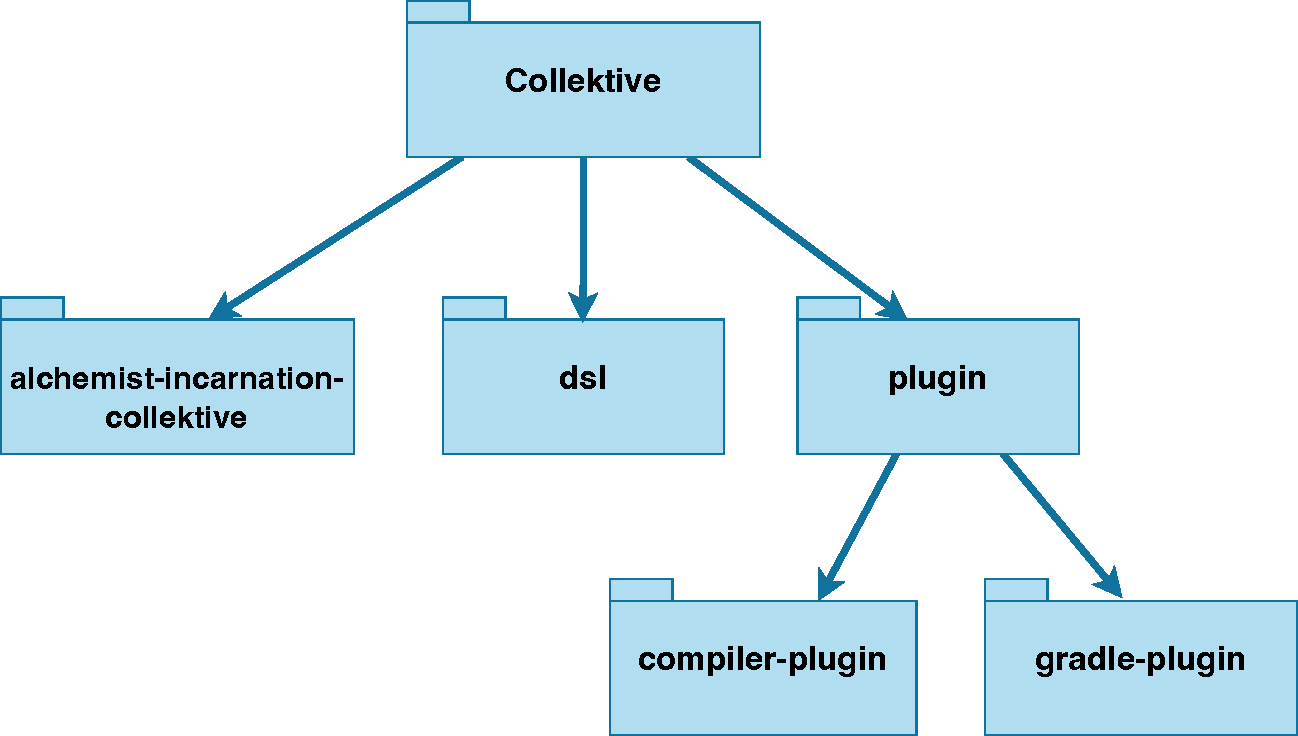
\includegraphics[width=0.7\textwidth]{figures/packages}
    \caption{Packages diagram of the Collektive project.}
    \label{fig:pacakges}
\end{figure}

Regarding the examples, there is a specific repository called \textbf{collektive-examples} that contains some samples of
aggregate programs to show how to use the \emph{Collektive} framework.

\section{DSL}
\label{sec:dsl}
In this thesis, the original implementation of the \ac{dsl} of \emph{Collektive} will be modified to allow the use of \xc{}
and to improve its performance.
The resultant \ac{dsl} is available at a public GitHub repository\footnote{\url{https://github.com/Collektive/collektive}}

A \ac{dsl} is a specialised programming language or language framework tailored to address the
requirements of a specific domain or problem area.
In contrast to general-purpose programming languages, which aim for versatility across various domains and problem categories,
DSLs are crafted to cater precisely to the demands of a particular application or system.
Consequently, general-purpose languages like Java typically exhibit greater complexity compared to \acp{dsl}.


\paragraph{Structure}
The \emph{Collektive}'s \ac{dsl} is composed of the following components:
\begin{itemize}
    \item \textbf{Path}: represents a specific point in the \ac{ast} of an aggregate program;
    \item \textbf{State}: is an association between a path and a value, it is used by the compiler plugin to
        keep track of the computational state of the device in order to provide the correct alignment of the nodes;
    \item \textbf{Field}: represents the \emph{computational field} used by aggregate constructs.
        It is a map of messages where the key is the identifier (ID) of the node, and the value is the associated message;
    \item \textbf{Message}: is an interface that represents the message exchanged between nodes, its concept will be explained in \ref{subsec:messages};
    \item \textbf{Network}: is the interface that represents the network used to manage the communication between devices;
    \item \textbf{Aggregate}: the actual core of the \ac{dsl}.
        It is also used to handle all the data needed for the computation; for example, the \emph{localId} and the \emph{state} of the device.
        It contains the primary functions on which the language is extended, such as \texttt{exchange}, \texttt{exchanging}, \texttt{repeat} and \texttt{repeating};
        To create an aggregate program, a function must extend this interface, in this way it will be possible to use the aggregate functions.
        It is also implemented the mechanism to handle the alignment of the functions used within the compiler plugin;
    \item \textbf{AggregateOperators}: contains the implementation of the functions created using the \texttt{exchange-exchanging} functions,
        such as \texttt{share}, \texttt{sharing} and \texttt{neighboringViaExchange}.
        Moreover, it contains the mechanism to manage the alignment of the fields used within the compiler plugin;
    \item \textbf{YieldSupport}: contains the \emph{Yielding Context} and the \emph{Yielding Result} for the ``yielding''
        operations, which means that the function operates on an initial value but possibly returns a different value;
    \item \textbf{Collektive}: is the entrypoint for creating a ``Collektive'' device, it must have a specific \emph{ID} and a
        \emph{network} to manage the communication between devices.
        The effective aggregate program is identified by the \emph{compute function}, which will be executed
    \item \textbf{AggregateResult}: is the result of one evaluation of the aggregate program, it contains the \emph{localId}
        of the node, the effective \emph{result} of the computation, the \emph{messages to send} to other devices and the \emph{new state} of the device;
\end{itemize}

\begin{figure}
    \centering
    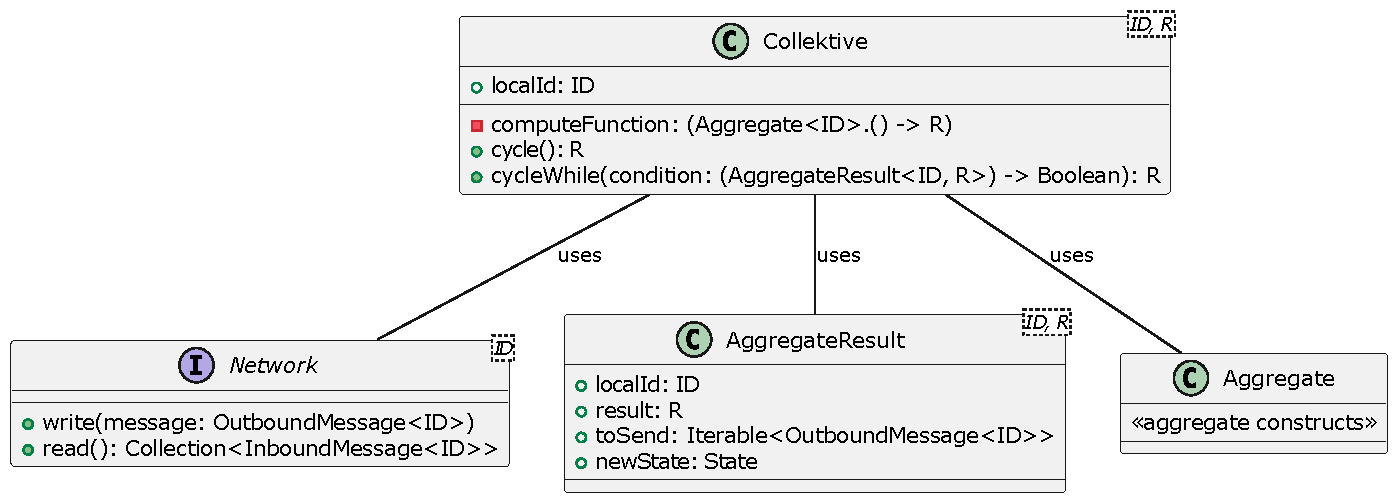
\includegraphics[width=\textwidth]{figures/entrypoint-class-diagram}
    \caption{Partial class diagram of the \ac{dsl}, highlighting the entrypoint.}
    \label{fig:entrypoint-class-diagram}
\end{figure}

\begin{figure}
    \centering
    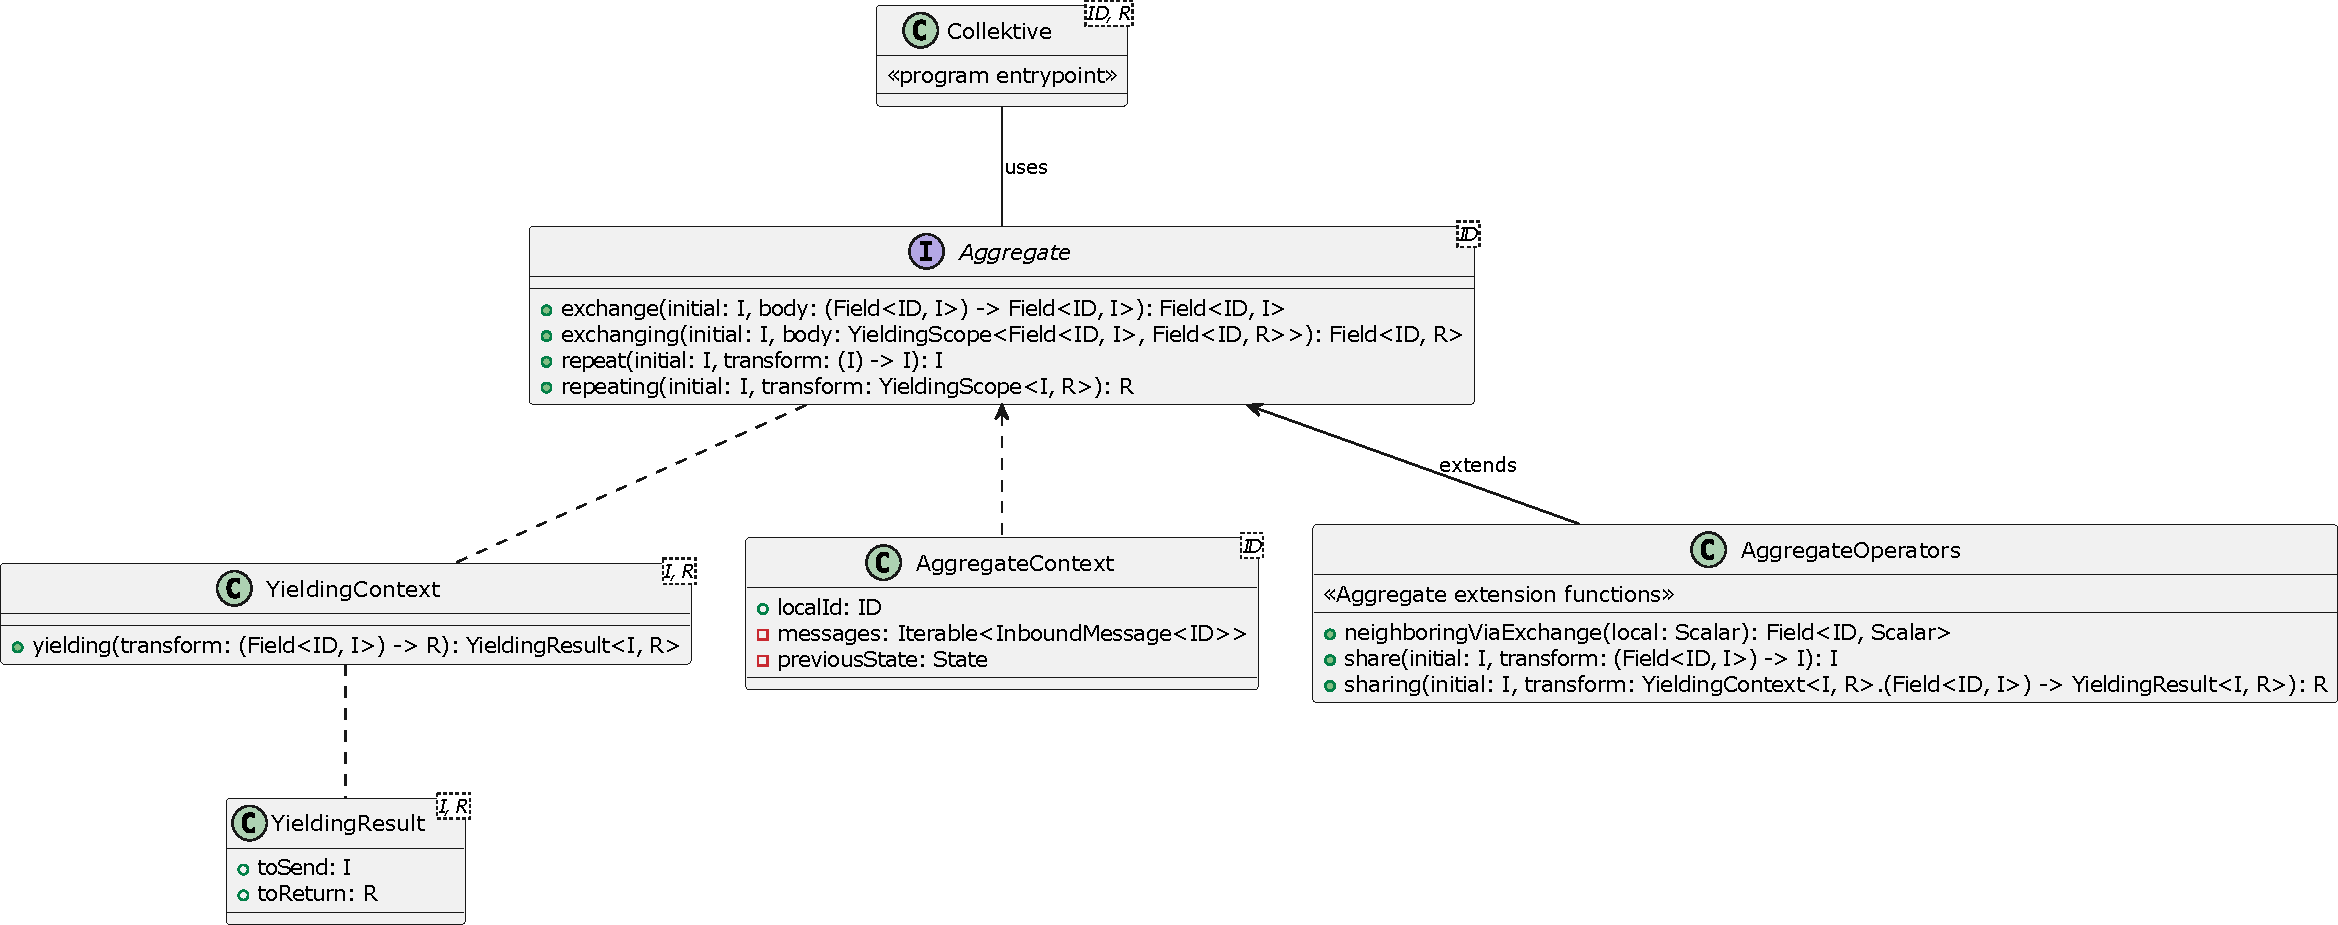
\includegraphics[width=\textwidth]{figures/aggregate-class-diagram}
    \caption{Partial class diagram of the \ac{dsl} structure, highlighting the \emph{Aggregate} section.}
    \label{fig:aggregate-class-diagram}
\end{figure}

In the class diagrams shown in \Cref{fig:aggregate-class-diagram} and \Cref{fig:entrypoint-class-diagram}, it is possible to see the main classes of the \ac{dsl}
introduced above and their relationships.
The Interface \emph{Aggregate} is implemented by the \emph{AggregateContext} class, which is used to handle the logic and the
computation of the main constructs of the \ac{dsl}.
This interface is then extended within \emph{AggregateOperators} to handle the logic of the functions created using the
\texttt{exchange-exchanging} functions.

\subsection{XC in Collektive}
\label{subsec:exchange-in-collektive}

Thanks to the design of \xc{}, it is possible to implement the methods proposed by \emph{field calculus}
(~\ref{par:syntax-of-field-calculus}) in terms of \emph{exchange} (~\ref{par:communication-in-xc}).
The syntax of \emph{XC} allows for sending messages to specific nodes, enabling the implementation of \emph{field calculus}
operations through message exchange.

The \emph{exchange} communication is based on \emph{anisotropic} communications, meaning that it has not the same properties
or characteristics in all directions (\Cref{fig:anisotropic}); therefore, messages have custom values sent to different neighbours.

\begin{figure}[h!]
    \centering
    \includegraphics[width=0.2\textwidth]{figures/anisotropic}
    \caption{Anisotropic communication.}
    \label{fig:anisotropic}
\end{figure}

This concept can be extended to the \texttt{share} function of field calculus, with the difference that the
operation of \texttt{share} is based on \emph{isotropic} communication, meaning that properties are uniform in all directions
(\Cref{fig:isotropic}); therefore, messages have the same value sent to all neighbours.

\begin{figure}[h!]
    \centering
    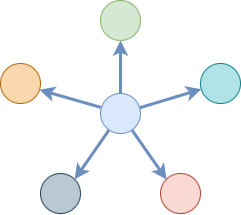
\includegraphics[width=0.2\textwidth]{figures/isotropic}
    \caption{Isotropic communication.}
    \label{fig:isotropic}
\end{figure}

All the \ac{dsl} has been modified to use \texttt{exchange} for the implementation of the other constructs such as \texttt{share}
and \texttt{nbr}, which is called \texttt{neighboring}.
Only the \texttt{rep} construct has not been implemented in terms of \texttt{exchange}, as it is a function that allows iterating
over oneself, it's better for neighbours not to receive messages of any kind, also for security and privacy reasons.
As the original implementation, it supports the evaluation of \emph{fields}.

\paragraph{Exchange}
The construct \texttt{exchange} provides
    \emph{(i)} access to neighbours' values,
    \emph{(ii)} persistence of information for subsequent executions,
    \emph{(iii)} communication with neighbours, and
    \emph{(iv)} compositional behaviour.

As seen in \ref{par:communication-in-xc}, the \texttt{exchange} function can send and return the same result, or it
can send a message and return a different result; both cases have been implemented.

The \texttt{exchange} takes an \emph{initial} value to use as a default, and a \emph{body} that defines an aggregate
function to be computed, as seen in the code snippet \ref{lst:exchange}, returning a \emph{field}.
When executing the aggregate program, it checks which messages have been received from the neighbours and applies the function,
generating a custom value for each neighbour.

In the early stages of the design of this function, potential problems that could arise during execution were evaluated,
such as the management of initialisation, i.e.\ the first round of message exchange.
Consider a network consisting of $n$ devices, in which all are considered as neighbours to each other.
The first device ($d_1$) to start within the network will certainly have a moment when it performs its first iteration ever.

The problem arises when the device $d_1$ has not yet received any messages, so it will not have neighbour values to perform
the calculation, thus creating a deadlock situation where it does not know the neighbourhood and does not know who to actually send a message to.
For this reason, it was necessary to implement a mechanism such that the device performs a first iteration on its initial value,
and send the message to the network without a specific recipient, so that the future ``neighbourhood'' can receive it and start a communication with $d_1$.
In this way, the next devices to ``wake up'' in the network will know that $d_1$ is present and will be able to communicate with it.

\begin{lstlisting}[language=kt,label={lst:exchange}, caption={The signature of the \texttt{exchange} function.}]
fun <Initial> exchange(
    initial: Initial,
    body: (Field<ID, Initial>) -> Field<ID, Initial>,
): Field<ID, Initial>
\end{lstlisting}

\paragraph{Share}
The \texttt{share} construct captures the space-time nature of field computation through observation of neighbours' values,
starting from an \emph{initial} value, it reduces to a single local value given a \emph{transform} function and updating and sharing to
neighbours of a local variable, then returns the punctual value evaluated from the transformation (\ref{lst:share}).

\begin{lstlisting}[language=kt,label={lst:share}, caption={The signature of the \texttt{share} function.}]
fun <ID : Any, Initial> Aggregate<ID>.share(
    initial: Initial,
    transform: (Field<ID, Initial>) -> Initial,
): Initial
\end{lstlisting}

As previously introduced, this construct can be expressed in terms of \texttt{exchange}.
What \texttt{share} differs from it is that \texttt{share} does not differentiate the result of the computation based on
the neighbour that sent the message; it sends it indiscriminately to all neighbours.

\paragraph{Neighboring}

The \emph{field calculus} construct \texttt{nbr} is implemented as \texttt{neighboring}, more precisely as \texttt{neighboringViaExchange}
due to its effective implementation based on the \texttt{exchanging} function.
The \texttt{neighboringViaExchange} construct is used to access the values of the neighbours.
It takes as parameter \emph{local} (\ref{lst:neighboring}), which can be an expression or a value, and returns a \emph{field} of the same input type.

\begin{lstlisting}[language=kt,label={lst:neighboring}, caption={The signature of the \texttt{neighboringViaExchange} function.}]
fun <ID : Any, Scalar> Aggregate<ID>.neighboringViaExchange(
    local: Scalar,
): Field<ID, Scalar>
\end{lstlisting}

\paragraph{Repeat}
The \texttt{repeat} function is the equivalent of the \texttt{rep} construct in \emph{field calculus}.
It models the state evolution over time, the value of \emph{initial} evolves at each execution depending on the \emph{transform} function,
and it returns the final value of the computation (\ref{lst:repeat}).

\begin{lstlisting}[language=kt,label={lst:repeat}, caption={The signature of the \texttt{repeat} function.}]
fun <Initial> repeat(
    initial: Initial,
    transform: (Initial) -> Initial,
): Initial
\end{lstlisting}

As previously mentioned, this function is not implemented in terms of \texttt{exchange}, because iterating over oneself
it is better not to send messages to neighbours, also for security and privacy reasons, its implementation will be explained in \ref{par:repeating}.

\subsection{Messages}
\label{subsec:messages}

The accurate modelling of message functionality is crucial for device communication.
Due to the different nature of messages supported, that is \emph{anisotropic} and \emph{isotropic} communication,
it has been necessary to create specific data classes for the handling of relative messages.

Previously, messages were sent to the network without considering the recipient, and the network was responsible for
delivering the message to all the neighbours that were interconnected.
Since the main feature of \texttt{exchange} is to send messages to specific neighbours with custom values, it is important
to ensure that unintended recipients do not receive the message.
Therefore, the old model of messages has been modified.

\begin{figure}
    \centering
    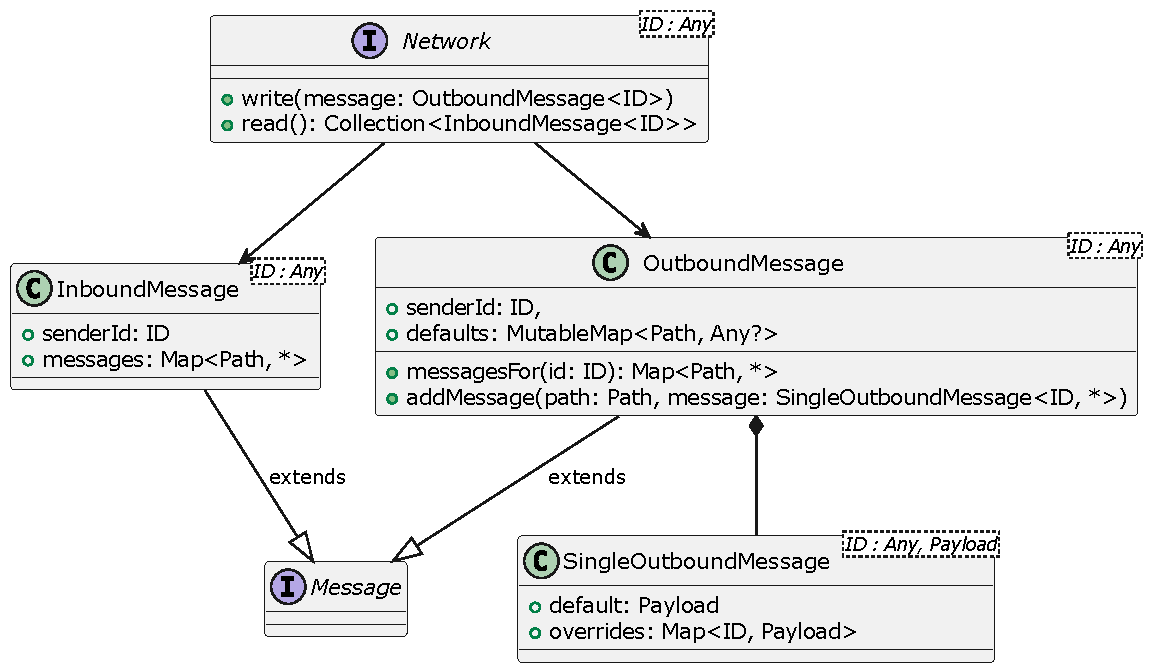
\includegraphics[width=\textwidth]{figures/messages-diagram}
    \caption{Class diagram of the network and messages stucture.}
    \label{fig:message-diagram}
\end{figure}

The \Cref{fig:message-diagram} shows the class diagram of the messages used in the \ac{dsl}, highlighting their relationships
and the inheritance of the \emph{Message} interface.
The concept and implementation of the messages will be explained in the following paragraphs.

\paragraph{OutboundMessage and SingleOutboundMessage}
It has been introduced the concept of \emph{OutboundMessage} (\Cref{lst:outbound}).
Its goal is to associate to the sender of the message, the messages to send to the neighbours.
With this implementation, it is possible to manage the messages for \emph{isotropic} and \emph{anisotropic} communication.
In this way, a device sends to the network just one \emph{OutboundMessage} that contains all the messages to send to the neighbours,
and also unburdens the payload of the network.

\begin{lstlisting}[language=kt,label={lst:outbound}, caption={Outbound message data class.}]
data class OutboundMessage<ID : Any>(
    expectedSize: Int,
    val senderId: ID,
) : Message
\end{lstlisting}

For what it concerns the \emph{anisotropic} communication, it is necessary to keep track of the identifier of the recipient
and the value associated with it, in order for the network to deliver the message to the correct neighbour.
This has been implemented with a map of \emph{overrides}, which associates to the recipient's identifier a specific value.

For the \emph{isotropic} communication, it is just necessary to keep track of the default value to send to all the neighbours
at a certain path of the computation.
This is used when there are no overrides for the recipient that is reading the messages received.
The network will be in charge to deliver the message to all the neighbours, so it is not necessary to keep track of the recipient's identifier.

\begin{lstlisting}[language=kt,label={lst:single}, caption={Single outbound message data class.}]
data class SingleOutboundMessage<ID : Any, Payload>(
    val default: Payload,
    val overrides: Map<ID, Payload>,
)
\end{lstlisting}

In summary, when a program is executed and a device has computed its function, it has to generate the messages to send to
the neighbours (so it's done inside the \texttt{exchange} function), it populates a \emph{SingleOutboundMessage} (\Cref{lst:single}),
that will be used to populate the \texttt{overrides} and the \texttt{default} maps of the \emph{OutboundMessage}.
At the end it is added to a list of \emph{OutboundMessage} and sent to the network.

\paragraph{InboundMessage}
The \emph{InboundMessage} is a data class (\Cref{lst:inbound}) modelled for the messages read from the network.
When reading the \emph{OutboundMessage}, there are some fields that are not needed, such as the receiver of the message,
which is the device itself, and is necessary to keep the default value or the override value.
To handle this, the \emph{InboundMessage} has been modelled to keep only the identifier of the sender and
a map of messages of \emph{Path} and the associated value.

\begin{lstlisting}[language=kt,label={lst:inbound}, caption={Inbound message data class.}]
data class InboundMessage<ID : Any>(
    val senderId: ID,
    val messages: Map<Path, *>,
) : Message
\end{lstlisting}

\subsection{Network}
\label{subsec:network}
The \emph{Network} has the task of managing only the reading and writing of messages in the network for a single device.
The actual implementation of the network is not managed by the \emph{Collektive} \ac{dsl}, but it is implemented in the
\emph{alchemist-incarnation-collektive} (\Cref{sec:incarnation}) module, which is used to run the aggregate programs
created with \emph{Collektive} on the simulator.

Inside the \ac{dsl}, it is used at the beginning of each iteration of the aggregate program to read the messages received from
other devices present in the network, and at the end of the iteration to write the messages to send to the other devices.
The network actually supports only the specific types of messages introduced in \Cref{subsec:messages}, due to the
concepts introduced by the study of \xc{} and field calculus.

\section{Plugin Extensions}
\label{sec:plugin-extensions}
In Kotlin, a plugin compiler extension refers to a mechanism that allows developers to extend or customise the behaviour
of the Kotlin compiler.
These extensions provide a way to hook into the compilation process and modify or enhance the way Kotlin code is compiled.

Developers can create their own compiler extensions by implementing the necessary interfaces or annotations defined by
the Kotlin compiler API.
These extensions can then be applied to Kotlin projects either globally or selectively, depending on the specific
requirements of the project.

In \ac{kmp} project development, the compiler undertakes a covert translation of Kotlin code into platform-specific code.
Prior to this translation, the Kotlin code undergoes conversion into an \ac{ir}.
This IR serves as a transitional format, facilitating the seamless creation of multiplatform compiler plugins.
Notably, this approach eliminates the necessity to develop separate plugins for each platform, thus optimising the
development process and fostering code reuse across varied environments.

Since the source code is fully accessible at compile time, it becomes feasible to analyse it to determine when the \emph{alignment}
of the functions is necessary; consequently, new code can be generated to ensure proper alignment.
Furthermore, because the generation process is based on the intermediate representation, it enables interoperability across
different project targets and devices running on the same platform.
Modifications to the plugin are applied during compile time, minimising any notable impact on execution time.
Lastly, users are shielded from the intricacies of alignment concerns, as the code generation process remains transparent to them.

\paragraph{Alignment}
\label{par:alignment}

The alignment in \emph{Collektive} was initially implemented inspecting and annotating the body of the (ex)\texttt{aggregate} functions;
none of the other functions were aligned.

In \emph{Collektive}, the alignment of the functions is made by the compiler plugin, which keeps track of the sequence of
functions called during the computation, using a custom stack.
Since initially the entrypoint of the \ac{dsl} was the \texttt{aggregate} function, the alignment was made by assuring
that a reference to the \emph{AggregateContext} was present, meaning that everything not related to the \ac{dsl} did not
require alignment.

By changing the main architecture of the \ac{dsl} to use \xc{}, it has been necessary to review the way the alignment was managed.

The alignment has been implemented in such a way that it also takes into account the functions from which an aggregate program is called.
For example (\Cref{lst:not-aligned}), we could have two different functions called \texttt{foo()} and \texttt{bar()} that both call the same aggregate program,
but in fact they are two different functions and therefore must be aligned differently.

\begin{lstlisting}[language=kt,label={lst:not-aligned}, caption={Example of two unaligned functions.}]
val x = 0
fun foo(aggregate: Aggregate<Int>) = aggregate.neighboringViaExchange(x)
fun bar(aggregate: Aggregate<Int>) = aggregate.neighboringViaExchange(x)
acProgram { foo(this) } shouldNot alignWith { bar(this) }
\end{lstlisting}

The alignment process follows a specific strategy.
Firstly, all function definitions are visited, and those involving aggregate computation are subject to alignment processing.
Next, for each candidate function, the plugin visits all call sites in the function's body and checks if the call has an
aggregate reference or is involved in an aggregate computation; meaning that it must have the \emph{Aggregate} type as
\texttt{extensionReceiver}, or \texttt{dispatchReceiver}, or one or more of the function's parameters.
If so, the plugin aligns the expression call.
While visiting the function definition, the plugin only aligns branch conditions that involve aggregate computation.
If a branch body does not involve aggregate computation, it will not be aligned.
This default alignment ensures that all branches follow the branch semantics of \ac{ac}.

All the functions visited are so pushed into a stack.
For each call to \emph{Aggregate} also push the name of the function in the stack, appending a value that represents the
occurrence of the function in the sequence of the computation.
When the control flow exits that function, the function name is popped from the stack.
The \emph{Path} generated is a string that represents the sequence of the functions called during the computation,
with the prepended calls of the non-Aggregate functions.

Since, during execution, the control of the effective alignment of two functions is done simply by comparing the two resulting strings,
the control of the whole path turns out to be less efficient than the initial one on the aggregate functions only.
However, this can be optimised by applying hashing to the paths, in order to reduce the comparison of strings with no deterministic length
to the comparison of fixed-length Longs.
Furthermore, the hashing approach would also be better from a privacy point of view.
Note that the paths' hashing should be implemented at plugin-level, this is because during the experiments it has been noticed
its implementation in the \ac{dsl} could lead to a significant increase in the execution time of the aggregate programs.

\section{Technologies}
\label{sec:technologies}

\paragraph{Kotlin Multiplatform}
\label{par:kotlin-multiplatform}

\emph{Kotlin} is a cross-platform, statically typed, general-purpose programming language with type inference.
It is designed to interoperate fully with Java, and the JVM version of its standard library depends on the Java Class Library.
However, \emph{Kotlin} is also used to target JavaScript, and native code (via LLVM).
The purpose of \ac{kmp} is to streamline the development process of cross-platform projects by minimizing
the effort required to write and upkeep identical code for various platforms, such as Android, iOS, full-stack web applications,
multiplatform libraries and its platform-specific implementations for \ac{jvm}, \ac{js}, and native code.

\ac{kmp} enables significant code reuse across multiple platforms, leading to faster development cycles,
reduced maintenance efforts, and improved code consistency.
\ac{kmp} supports compilation targets for various platforms, including Kotlin/JVM for backend and desktop applications,
Kotlin/JS for web applications, and Kotlin/Native for Android, iOS, and other native platforms.
Developers specify the compilation targets in the Gradle configuration to generate platform-specific binaries.

\paragraph{Kotest}
\emph{Kotest} is a powerful testing framework for Kotlin that provides a flexible and expressive way to write tests for Kotlin projects.
It offers a rich set of features and utilities to make testing easier, more concise, and more effective.

\emph{Kotest} provides a wide range of built-in matchers and assertion functions for common test scenarios, such as equality
checks, collection assertions, exception handling, and more.
These utilities make it easy to write expressive and accurate assertions without boilerplate code.
Some test examples will be shown in \Cref{sec:tests}.

\paragraph{Gradle}
Gradle is a powerful build automation tool and dependency management system used primarily for Java, Kotlin, and Groovy projects.
It is designed to be highly flexible, scalable, and efficient, making it a popular choice among developers and
organisations for building and managing software projects.

Gradle uses a declarative \ac{dsl} based on Groovy or Kotlin to define build scripts.
This DSL allows developers to express build configurations, tasks, dependencies, and plugins in a concise and readable format.
Gradle build scripts are typically named build.gradle and are written in Groovy or Kotlin.

Gradle organises the build process around tasks, which are units of work that perform specific actions, such as compiling
source code, running tests, or generating documentation.
Developers can define custom tasks and dependencies between tasks in the build script, allowing for fine-grained control over the build process.
Gradle executes tasks in parallel when possible, leveraging multi-threading to improve build performance.

\section{Implementation}
\label{sec:implementation}
In this section, the actual implementation of the \ac{dsl}'s functionalities will be examined, with code examples and explanations
regarding the implementation choices and the problems encountered during development.

\subsection{Fields}
\label{subsec:fields}
About the manipulation of the \emph{neighbouring values} introduced in \Cref{par:data-types}, it has been implemented
the concept of \emph{Field} to handle the data structure to send between neighbours, and relatives functions to manipulate it.

The \emph{Field} keeps track of the identifier of the device (\texttt{localId}) and the value associated with it
(\texttt{localValues}) and eventually a map that associates the identifiers of the neighbours to their exchanged local values.
In order to improve the performance of the system, a version of the \emph{Field} has been implemented, called \emph{ConstantField}.
This is used to implement the mechanism of isotropic message, which is often used in the communications.
The \emph{ConstantField} keeps track of the identifiers of the neighbours with which to communicate in a list and the value to send only once,
whilst the \emph{Field} keeps track of the value to send for each neighbour as a map, which is more expensive in terms of performance.

\subsection{Collektive entrypoint}
\label{subsec:collektive-entrypoint}
The public entrypoint of the \ac{dsl} is the \emph{Collektive} class, which can be interpreted as a device that can
execute an aggregate program.

As seen in the code snippet \ref{lst:collektive}, the \emph{Collektive} class takes as parameters the \emph{localId} of the device,
the \emph{network} used to manage the communication between devices, and the \emph{computeFunction} that will be executed
when the device is ready to compute the aggregate program.

\begin{lstlisting}[language=kt,label={lst:collektive}, caption={The signature of the \texttt{Collektive} class.}]
class Collektive<ID : Any, R>(
    val localId: ID,
    private val network: Network<ID>,
    private val computeFunction: Aggregate<ID>.() -> R,
)
\end{lstlisting}

The aim of this class is to manage the logic and the effective execution of the rounds of the aggregate program passed as a parameter.

It provides two main functions that will be called in the incarnation to execute the program:
\begin{itemize}
    \item \texttt{cycle}: applies once the \emph{computeFunction} and returns the result of the computation;
    \item \texttt{cycleWhile}: applies the \emph{computeFunction} while the condition passed as parameter is satisfied,
        and returns the result of the computation.
\end{itemize}

Both functions are implemented through a private function \texttt{executeRound}, which effectively calls the aggregate program,
managing the result obtained and updating the internal state of the device.

There are two types of aggregate programs: one that uses the \emph{Network} and one that does not, but directly takes
a set of \emph{InboundMessage}.

\begin{lstlisting}[language=kt,label={lst:aggregate}, caption={The signature of the \texttt{aggregate program}.}]
fun <ID : Any, R> aggregate(
        localId: ID,
        network: Network<ID>,
        previousState: State = emptyMap(),
        compute: Aggregate<ID>.() -> R,
    ): AggregateResult<ID, R> = with(AggregateContext(localId, network.read(), previousState)) {
        AggregateResult(localId, compute(), messagesToSend(), newState()).also {
            network.write(it.toSend)
        }
    }
\end{lstlisting}

The code seen in \ref{lst:aggregate} is the implementation of the \texttt{aggregate} function that relies on the \emph{Network}.
Taking the \emph{AggregateContext} as context with the messages read from the network and the previous state of the
device, it applies the \emph{compute} function.
The result of the computation is then returned as an \emph{AggregateResult} (\Cref{lst:aggregateresult}), which contains the \emph{localId} of the device,
the effective \emph{result} of the computation, the \emph{messages to send} to other devices and the \emph{new state} of the device.
Finally, the messages to send are written to the network.
This is the function called from the \texttt{executeRound} function.

\begin{lstlisting}[language=kt,label={lst:aggregateresult}, caption={The signature of the \texttt{aggregate result}.}]
data class AggregateResult<ID : Any, R>(
    val localId: ID,
    val result: R,
    val toSend: OutboundMessage<ID>,
    val newState: State,
)
\end{lstlisting}

\subsection{Yielding Support}
\label{subsec:yielding-support}
To operate on an initial value but possibly return a different value, it has been introduced
the concept of \emph{yielding}.
The operations of yielding are used to operate on an initial value, which is usually exchanged with the neighbours,
but possibly return a different value to the caller.
This operation is executable on the \texttt{exchanging}, \texttt{sharing} and \texttt{repeating} methods, or it can be omitted
in case the value obtained from the operation is to be returned.
Those constructs will be explained in detail in the sections \ref{subsec:aggregate-context} and \ref{subsec:aggregate-operators}.

\begin{lstlisting}[language=kt,label={lst:yieldingcontext}, caption={The signature of the \texttt{yielding context} class.}]
class YieldingContext<Initial, Return> {
    fun Initial.yielding(toReturn: () -> Return): YieldingResult<Initial, Return> =
        YieldingResult(this, toReturn())
}
\end{lstlisting}

\subsection{Aggregate Context}
\label{subsec:aggregate-context}

The \emph{AggregateContext} class is the class that effectively has the implementation of the basic constructs inside the \ac{dsl}.
Internally, it keeps track of the {stack}, the state, and the messages that need to be sent by that device.

\paragraph{Exchange}
There are two versions of this construct: one that has the same type of value of the field in output as the one in input (\Cref{lst:exchangeImpl}),
and one in which they differ (\Cref{lst:exchanging}).
The \texttt{exchange} construct is the one that represents the communication in which $e_r$ (the value to return)
and $e_s$ (the value to send) coincide, as illustrated in \ref{par:communication-in-xc}.

\begin{lstlisting}[language=kt,label={lst:exchangeImpl},caption={The implementation of the \texttt{exchange} function.}]
override fun <X> exchange(initial: X, body: (Field<ID, X>) -> Field<ID, X>): Field<ID, X> =
        exchanging(initial) { field -> body(field).run { yielding { this } } }
\end{lstlisting}

The \texttt{exchange} therefore simply calls the \texttt{exchanging}, but as the context of the yielding it passes the
field on which the computation has been executed.

The real functioning of \xc{} relies in the \texttt{exchanging} implementation, which is the one that effectively manages
the actual logic of the computation and the messages to send to the neighbours.

In the \Cref{lst:exchanging} snippet is shown how the \texttt{exchanging} function is implemented.
First, it takes the current path from the stack kept inside the context and the messages received whose path is the same,
so that it is possible to evaluate only aligned messages.
Then it takes the state of the device at the current path, using the initial value passed as a parameter in case there is no previous state.
A new field is then created on which to perform the computation, starting from the value of the state and the messages received at the current path.
If there are no messages received at the current path, simply there will be an empty map of messages.
The new field is then passed to the body passed in input, along with a new \emph{yielding context}, on which the computation is effectively executed.
The result obtained from the computation is then returned and, depending on what has been passed as a yielding context in the body,
the value is sent to the neighbours, which can be either the result of the computation (in the \texttt{retsend} case) or a value of a different type.

A message of type \emph{SingleOutboundMessage} is created, populated with the value obtained from the application to the field
of the aggregate function put as the default value, while as an override it is evaluated what type of field has been
obtained from the computation, and based on this the value is sent to the neighbours.
If the field is of a constant type, the map of overrides will be empty, otherwise the value obtained from the computation
is sent, excluding the value of the device itself.
A check is made to verify that there are no messages aligned with the same path, as this could cause an alignment conflict.
Finally, the message is added to the map of messages to be sent, and the state of the device is updated with the value obtained from the computation.

\begin{lstlisting}[language=kt,label={lst:exchanging},caption={The implementation of the \texttt{exchanging} function.}]
override fun <Init, Ret> exchanging(
    initial: Init,
    body: YieldingScope<Field<ID, Init>, Field<ID, Ret>>,
): Field<ID, Ret> {
    val path = stack.currentPath()
    val messages = messagesAt<Init>(path)
    val previous = stateAt(path, initial)
    val subject = newField(previous, messages)
    val context = YieldingContext<Field<ID, Init>, Field<ID, Ret>>()
    return body(context, subject).also {
        val message = SingleOutboundMessage(
            it.toSend.localValue,
            when (it.toSend) {
                is ConstantField<ID, Init> -> emptyMap()
                else -> it.toSend.excludeSelf()
            },
        )
        check(!toBeSent.messages.containsKey(path)) {
            """
                Aggregate alignment clash by multiple aligned calls with the same path: $path.
                The most likely cause is an aggregate function call within a loop
            """.trimIndent()
        }
        toBeSent = toBeSent.copy(messages = toBeSent.messages + (path to message))
        state += path to it.toSend.localValue
    }.toReturn
}
\end{lstlisting}

\paragraph{Repeat}
\label{par:repeating}
The \texttt{repeat} construct is the one that models the state evolution over time.
It is not implemented in terms of \texttt{exchange}, as it is a function that allows iterating over oneself,
it can directly update its internal state without sending messages to neighbours.

The \texttt{repeat} construct takes as parameters the \emph{initial} value and the \emph{transform} function, and returns the
final value of the computation of the same type as the initial.
To return a different type, it has been implemented the \texttt{repeating} function, as for the \texttt{exchange} construct,
using the \emph{yielding support} (\Cref{lst:repeating}).

\begin{lstlisting}[language=kt,label={lst:repeating},caption={The implementation of the \texttt{repeating} function.}]
 override fun <Initial, Return> repeating(
    initial: Initial,
    transform: YieldingScope<Initial, Return>,
): Return =
     transform(YieldingContext(), stateAt(stack.currentPath(), initial))
        .also { state += stack.currentPath() to it.toReturn }
        .toReturn
\end{lstlisting}

The \texttt{transform} function is applied to the state of the device, checking whether there are already values to use
on the stack, or using the initial value passed as a parameter.
After the computation, the stack is updated with the new value obtained from the computation, and the result is returned,
depending on the yielding context passed in the body of the function.

\subsection{Aggregate Operators}
\label{subsec:aggregate-operators}
The functions implemented using the \texttt{exchange} mechanism are situated in a separate class called \emph{AggregateOperators}.

\paragraph{Share}
The \texttt{share} is also implemented with the \emph{yielding support} mechanism, using the same base concept as in the
\texttt{exchange} and \texttt{repeat} functions.
This means that it is possible to operate on an initial value, but possibly return a different value, as seen in the code snippet \ref{lst:sharing}.

\begin{lstlisting}[language=kt,label={lst:sharing},caption={The implementation of the \texttt{sharing} function.}]
fun <ID : Any, Initial, Return> Aggregate<ID>.sharing(
    initial: Initial,
    transform: YieldingContext<Initial, Return>.(Field<ID, Initial>) -> YieldingResult<Initial, Return>,
): Return = exchanging(initial) { field: Field<ID, Initial> ->
    with(YieldingContext<Initial, Return>()) {
        val result: YieldingResult<Initial, Return> = transform(field)
        field.map { result.toSend }.yielding {
            field.map { result.toReturn }
        }
    }
}.localValue
\end{lstlisting}

Given the \emph{isotropic} nature of communication through \texttt{share}, the implementation via \texttt{exchange} is done
in such a way as to send the same value to all neighbours, so there is no need to keep track of who sent the message,
but only to send it to all neighbours.
The value sent to the neighbours can be the value expressed thanks to the \texttt{yielding} function, or the value obtained
from the computation, if the \texttt{share} function is used.

\paragraph{NeighboringViaExchange}
The \texttt{neighboringViaExchange} construct is used to access the values of the neighbours.
It takes as parameter \emph{local}, which can be an expression or a value, and returns a \emph{field} of the same type (\ref{lst:neighboringViaExchange}).

\begin{lstlisting}[language=kt,label={lst:neighboringViaExchange},caption={The implementation of the \texttt{neighboringViaExchange} function.}]
fun <ID : Any, Scalar> Aggregate<ID>.neighboringViaExchange(local: Scalar): Field<ID, Scalar> =
    exchanging(local) { toYield ->
        toYield.mapToConstantField(local).yielding { toYield }
    }
\end{lstlisting}

As said in \Cref{par:communication-in-xc}, the \texttt{nbr} construct is a peculiar case of \texttt{exchange}, in which
the value of the expression evaluated is sent to neighbours and the values received from them are returned as a field.
In this way, it provides a view of the values computed by the neighbours.
Thus, its implementation consists of a call to the \texttt{exchanging} function, made in such a way as to send the value
evaluated to the neighbours and return the values received from them as a field.

\section{Alchemist Incarnation}
\label{sec:incarnation}
An ``incarnation'' serves as the interpreter enabling the \emph{Alchemist Simulator} to comprehend and accurately execute a language.
Specifically designed for \emph{Collektive} ~\footnote{\url{https://github.com/Collektive/collektive}},
this incarnation employs reflections to locate the aggregate entry point and dictates the methodology for each iteration of the aggregate program.
Similar to other Alchemist incarnations like \texttt{alchemist-incarnation-scafi} and \texttt{alchemist-\\incarnation-protelis},
it has been implemented to launch simulations through Gradle tasks.

The goal is to ensure that the new implementation is still compatible with the simulator and that it can be used to run simulations without any issues.

To achieve this, it was necessary to modify the \emph{Collektive Device} previously implemented, to make it compatible
with the new implementation of the network and the related message exchange.
Furthermore, the functioning of the \emph{Distance Sensor} has been updated, and a new sensor has been added to detect
the properties of the molecule of interest (\emph{Local Sensing}).
To run simulations starting from a YAML file with the appropriate \emph{Alchemist} configuration, it was necessary to
create a class that reads the configuration and sets up the simulation.

The \emph{Alchemist} simulator is based on a system of actions and reactions, so to run an incarnation, it is necessary
to define an action that represents the behaviour of the nodes.
In this case, it is \texttt{RunCollektiveProgram} (\Cref{par:run-collektive-program}).

The incarnation is therefore provided to manage the behaviour of the molecules or nodes, so overriding the methods
provided by the \texttt{Alchemist} library.

\begin{figure}
    \centering
    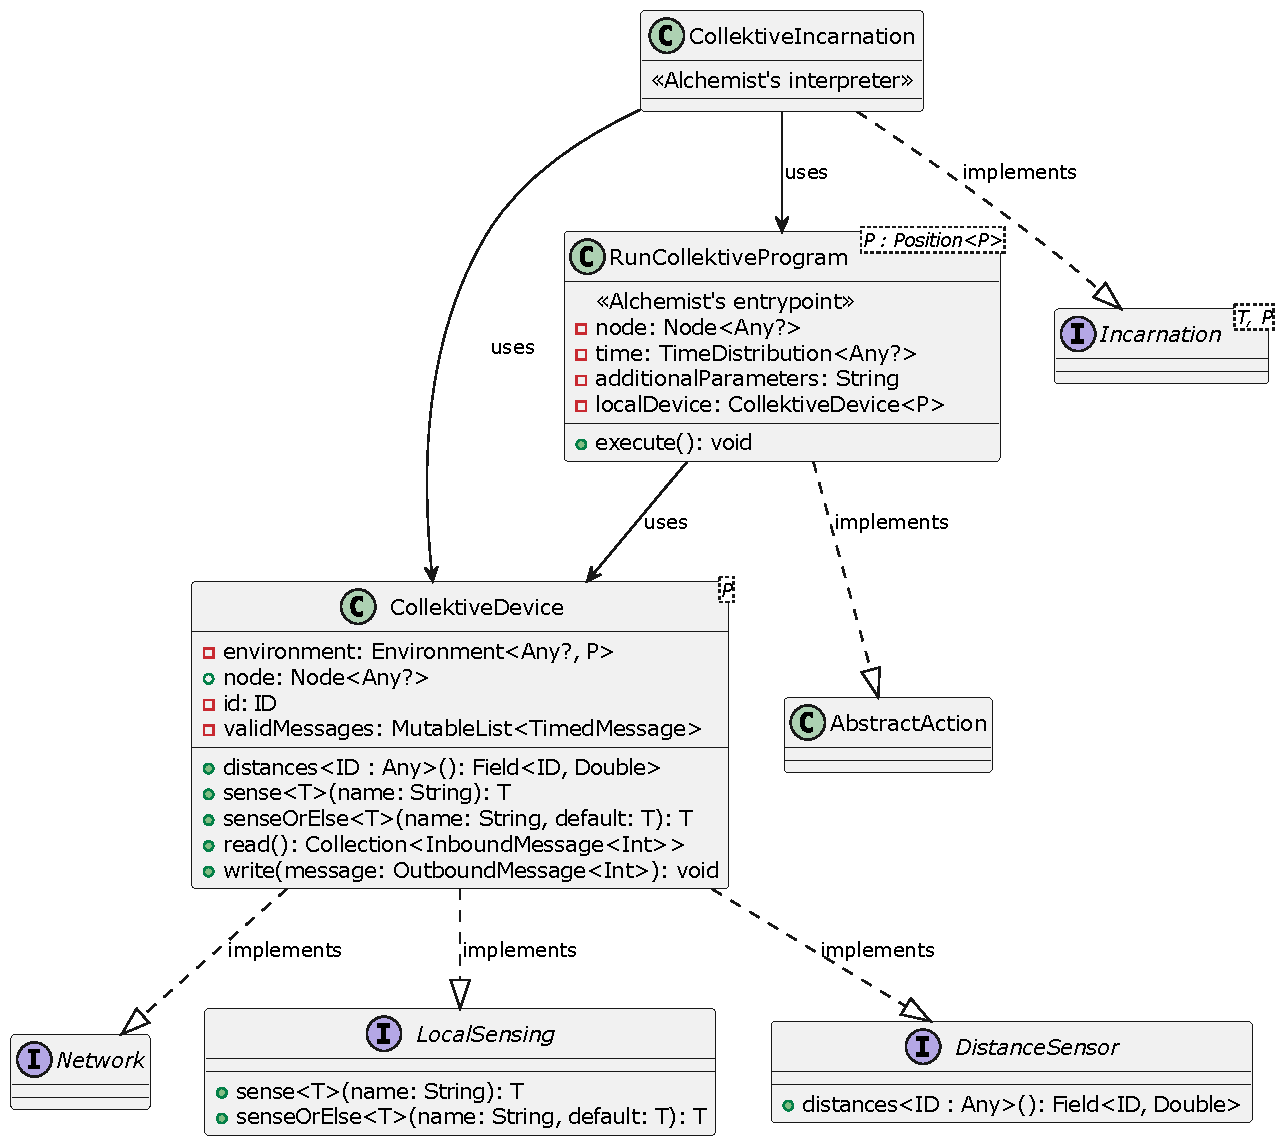
\includegraphics[width=\textwidth]{figures/incarnation-class-diagram}
    \caption{Class diagram of the \emph{Alchemist Incarnation} module.}
    \label{fig:incarnation-class-diagram}
\end{figure}

In the \Cref{fig:incarnation-class-diagram} is shown the structure of the \emph{Alchemist Incarnation} module.
It highlights the fact that the \emph{CollektiveDevice} has to manage the specific sensors and actuators and implement
the network from the device's perspective to manage messages sent and received from neighbours.

\paragraph{CollektiveDevice}
The \emph{CollektiveDevice} is a representation of the device in the \emph{Alchemist Simulator}.
Its purpose is to manage specific sensors and actuators and implement the network from the device's perspective to
manage messages sent and received from neighbours.

A device must have the \emph{environment} in which it is located, the \emph{node} property to be represented in the environment,
a specific \emph{ID} that is the same of the node, a \emph{retention time} for messages which can be null if it is necessary
to keep all messages.
It must extend the eventual sensors and the network to manage the communication with the neighbours.

To keep track of the time when the messages arrived and thus to be able to discard them after a certain time,
a private data class \texttt{TimedMessage} has been created that associates the time when each message arrived with the message itself.
In this way, in the effective implementation of the \texttt{read} function of the network, it is possible
to discard the messages that arrived before a certain time, and thus are no longer valid.

\begin{lstlisting}[language=kt,label={lst:read},caption={The implementation of the \texttt{read} function of the \texttt{Network}.}]
override fun read(): Collection<InboundMessage<Int>> =
    when {
        validMessages.isEmpty() -> emptySet()
        retainMessagesFor == null ->
            validMessages.map { it.payload }.also { validMessages.clear() }
        else -> {
            validMessages.retainAll { it.receivedAt + retainMessagesFor >= currentTime }
            validMessages.map { it.payload }
        }
    }
\end{lstlisting}

In the \Cref{lst:read} snippet is shown how the \texttt{read} function of the network is implemented.
It checks if the \emph{retainMessagesFor} property is null, meaning that it is necessary to keep all the messages,
and in this case it returns the valid messages and clears the set, otherwise it retains only the messages that arrived
after a certain time and returns them converted to a set of \emph{InboundMessage}.

The \texttt{write} function is the one that effectively sends the messages to the network, it has to manage the messages
taken as input from the \emph{aggregate context}.
It gets the neighbours of the device, and for each of them it creates an \texttt{InboundMessage} that the neighbour will read.
It has been noticed that the implementation of the network's functions affects the performance of the aggregate programs,
so it has been necessary to optimise the code to improve the performance.

If present, sensors and actuators are implemented within the \emph{CollektiveDevice} class.
For instance, in this particular implementation, the \emph{CollektiveDevice} incorporates a \emph{DistanceSensor} responsible for
measuring the distance between the device and its neighbouring entities and a \emph{LocalSensing} sensor for detecting the
value of the molecule of interest.
The method of the \emph{DistanceSensor} is realised as an aggregate extension function, utilised for gauging the spatial
separation between the device and its neighbours via the \texttt{neighboringViaExchange} construct.
This method acquires the positions of neighbouring devices and computes the distances between them, as exemplified in code snippet \ref{lst:distance}.
The utility of this function extends to other aggregate programs by virtue of employing the \texttt{DistanceSensor} interface as a contextual receiver.

\begin{lstlisting}[language=kt,label={lst:distance},caption={The implementation of the \texttt{distance} function.}]
override fun <ID : Any> Aggregate<ID>.distances(): Field<ID, Double> =
    environment.getPosition(node).let { nodePosition ->
        neighboringViaExchange(nodePosition).map { position -> nodePosition.distanceTo(position) }
    }
\end{lstlisting}

\paragraph{RunCollektiveProgram}
\label{par:run-collektive-program}
The \emph{RunCollektiveProgram} is an action for the \emph{Alchemist Simulator} that runs a \emph{Collektive} program.
It takes the \emph{node} on which executes the action, the time distribution of the events and the \emph{additional parameters}
which is the path where the aggregate program to execute is located.

This action is designed to accept the program to be executed as a parameter of the YAML and instantiate it via reflection.
Reflection stands as a potent feature within Kotlin, facilitating developers in the examination and manipulation of a program's structure during runtime.
This capability enables access and modification of properties, methods, and types within a program, alongside dynamic invocation of functions and constructors.
The reflection mechanism facilitates the retrieval of contexts passed to the aggregate program.

To instantiate the program, it is necessary to obtain any contexts passed through the context receivers or as parameters,
instantiate them, and pass them to the program, along with the aggregated context required for its execution.
This is where the behavior of the node is effectively defined when the action is executed, which calls the \texttt{cycle} method of \texttt{Collektive}.

Additionally, the implementation of a private cache has been essential for storing associated parameters of the aggregate program.
This measure aims to circumvent the recurrent utilisation of the reflection mechanism during program execution, a practice known to substantially impact performance.

\paragraph{CollektiveIncarnation}
The \emph{Collektive Incarnation} is an interpreter that enables the \emph{Alchemist Simulator} to understand and execute
the aggregate program written in the \ac{dsl}.
The incarnation is therefore provided to manage the behaviour of the molecules or nodes, so overriding the methods
provided by the \texttt{Alchemist} library.
It can evaluate runtime properties passed through the simulator, which are lambda functions.
A cache system has been put in place to prevent the need for re-evaluating molecule's properties and concentration each time,
activating only during system updates.
This was necessary due to performance issues.

\paragraph{Running the simulations}
To execute the simulations outlined in the subsequent chapter (\Cref{sec:alchemist-simulations}), the creation of a
configuration file in YAML format, adhering to \emph{Alchemist}'s YAML specifications, becomes imperative.
Within the YAML configuration file, parameters defining the simulation are delineated, encompassing variables such as
the node count, environmental characteristics, network model, and the pathway of the aggregate program slated for execution.
Following the creation of the configuration file, simulation execution becomes feasible through Gradle tasks.

In the yaml configuration file, it is possible to specify the parameters of the simulation, such as the number of nodes,
the type of environment, the network model, and the path of the aggregate program to run.
Once the configuration file has been created, it is possible to run the simulation through Gradle tasks.

There are two types of Gradle tasks for each simulation: one is for testing purposes (\texttt{runTaskNameBatch}), and the other
one is to run the simulation with the \emph{Alchemist} GUI (\texttt{runTaskNameGraphic}).
Tasks are configured in the \texttt{build.gradle} file, and the parameters in which the two types of tasks differ are
passed as arguments to the task.